\documentclass{article}

% Reverse the commented/uncommented lines below to switch
% between pdflatex and xelatex
%
\usepackage[utf8]{inputenc}
%\usepackage{fontspec}
%usepackage{xunicode}

\usepackage{float}
\usepackage{algorithm}
\usepackage[noend]{algpseudocode}
\usepackage{graphicx}
\usepackage{color}
\usepackage{xy}
\usepackage{url}
\usepackage{afterpage}
\usepackage{fullpage}

\newcommand{\set}[1]{\{#1\}} 
\newcommand{\setof}[2]{\{\,{#1}|~{#2}\,\}}
\newcommand{\compl}[1]{\overline{#1}}

\newcommand{\C}{\mathbb{C}} 
\newcommand{\N}{\mathbb{N}} 
\newcommand{\Q}{\mathbb{Q}} 
\newcommand{\R}{\mathbb{R}} 
\newcommand{\Z}{\mathbb{Z}}

\newcommand{\Continue}{\textbf{continue}}
\newcommand{\attr}{\ensuremath{\leftarrow} }
\newcommand{\nullvalue}{\ensuremath{\bot}}
\newcommand{\maxLvl}{\ensuremath{\mathrm{MaxLvl}}}
\newcommand{\maxInt}{\ensuremath{\mathrm{MaxInt}}}
\newcommand{\minInt}{\ensuremath{\mathrm{MinInt}}}

\begin{document}

\title{The Adaptive Priority Queue with Elimination and Combining}
\author{Irina Calciu, Hammurabi Mendes, and Maurice Herlihy\\
Department of Computer Science\\
Brown University\\
115 Waterman St., 4th floor\\
Providence RI -- USA\\
\texttt{\{irina,hmendes,mph\}@cs.brown.edu}
}

\maketitle

\begin{abstract}
Priority queues are fundamental abstract data structures, often used to manage limited resources in parallel programming. Several proposed parallel priority queue implementations are based on skiplists, harnessing the potential for parallelism of the \texttt{add()} operations. In addition, methods such as Flat Combining have been proposed to reduce contention by batching together multiple operations to be executed by a single thread. While this technique can decrease lock-switching overhead and the number of pointer changes required by the \texttt{removeMin()} operations in the priority queue, it can also create a sequential bottleneck and limit parallelism, especially for non-conflicting \texttt{add()} operations.

In this paper, we describe a novel priority queue design, harnessing the scalability of parallel insertions in conjunction with the efficiency of batched removals. Moreover, we present a new elimination algorithm suitable for a priority queue, which further increases concurrency on balanced workloads with similar numbers of \texttt{add()} and \texttt{removeMin()} operations. We implement and evaluate our design using a variety of techniques including locking, atomic operations, hardware transactional memory, as well as employing adaptive heuristics given the workload.
\end{abstract}

\section{Introduction}
\label{Sec-Introduction}

A priority queue is a fundamental abstract data structure that stores a set of keys (or a set of key-value pairs), where keys represent priorities. It usually exports two main operations: \texttt{add()}, to insert a new item in the priority queue, and \texttt{removeMin()}, to remove the first item (the one with the highest priority). Parallel priority queues are often used in discrete event simulations and resource management, such as operating systems schedulers. Therefore, it is important to carefully design these data structures in order to limit contention and improve scalability. Prior work in concurrent priority queues exploited parallelism by using either a heap~\cite{pqhunt} or a skiplist~\cite{Lotan2000} as the underlying data structures. In the skiplist-based implementation of Lotan and Shavit~\cite{Lotan2000} each node has a ``deleted'' flag, and processors contend to mark such ``deleted'' flags concurrently, in the beginning of the list. When a thread logically deletes a node, it tries to remove it from the skiplist using the standard removal algorithm. A lock-free skiplist implementation is presented in \cite{pqsundelltsigas}. 

However, these methods may incur limited scalability at high thread counts due to contention on shared memory accesses. Hendler et al.~\cite{Hendler2010} introduced Flat Combining, a method for batching together multiple operations to be performed by only one thread, thus reducing the contention on the data structure. This idea has also been explored in subsequent work on delegation~\cite{Metreveli2012,CalciuDHHKMM13}, where a dedicated thread called a \emph{server} performs work on behalf of other threads, called \emph{clients}. Unfortunately, the server thread could become a sequential bottleneck. A method of combining delegation with elimination has been proposed to alleviate this problem for a stack data structure~\cite{HotPar13Stack}. Elimination~\cite{Hendler2010a} is a method of matching concurrent inverse operations so that they don't access the shared data structure, thus significantly reducing contention and increasing parallelism for otherwise sequential structures, such as stacks. An elimination algorithm has also been proposed in the context of a queue~\cite{Moir2005}, where the authors introduce the notion of \emph{aging operations} - operations that wait until they become suitable for elimination.


In this paper, we describe, to the best of our knowledge, the first elimination algorithm for a priority queue.
Only \texttt{add()} operations with values smaller than the priority queue minimum value are allowed to eliminate. However, we use the idea of aging operations introduced in the queue algorithm to allow \texttt{add()} values that are \emph{small enough} to participate in the elimination protocol, in the hope that they will soon become eligible for elimination.
We implement the priority queue using a skiplist and we exploit the skiplist's capability for both operations-batching and disjoint-access parallelism. 
\texttt{RemoveMin()} requests can be batched and executed by a server thread using the combining/delegation paradigm. 
 \texttt{Add()} requests with high keys will most likely not become eligible for elimination and need to be inserted in the skiplist, sometimes requiring expensive traversals towards the end of the data structure to do so. Therefore, these operations represent a bottleneck for the server and a missed opportunity for parallelism. To alleviate these issues, we split the underlying skiplist into two parts: a \emph{sequential} part, managed by the server thread and a \emph{parallel} part, where high-valued \texttt{add()} operations can insert their arguments in parallel. Our design reduces contention by performing batched sequential \texttt{removeMin()} and small-value \texttt{add()} operations, while also leveraging parallelism opportunities through elimination and parallel high-value \texttt{add()} operations. We show that our priority queue outperforms prior algorithms in high contention workloads on a SPARC Niagara II machine. Finally, we explore whether the use of hardware transactions could simplify our design and improve throughput. Unfortunately, machines that support hardware transactional memory (HTM) are only available for up to four cores (eight hardware threads), which is not enough to measure scalability of our design in high contention scenarios. Nevertheless, we showed that a transactional version of our algorithm is better than a non-transactional version on a Haswell four-core machine. We believe that these preliminary results will generalize to machines with more threads with support for HTM, once they become available. In summary, our main contributions are:
\begin{itemize}
\item We propose the first elimination algorithm for a priority queue, consisting of (1)~\emph{immediate elimination}, where suitable \texttt{add()} and \texttt{removeMin()} operations exchange arguments; and (2)~\emph{upcoming elimination}, where \texttt{add()} operations with small keys, yet not suitable for elimination, wait some time until either they become suitable or time out.
\item We describe a scalable design for a priority queue based on our elimination algorithm and the delegation/combining paradigm introduced by prior work.
\item We augment our priority queue design with an adaptive component that allows it to perform combining and elimination efficiently, while also allowing \texttt{add()} operations not involved in the elimination to insert in parallel. 
\item We analyze how hardware transactions could be used to simplify and improve our initial design and show performance results on a Haswell machine with transactional memory enabled. 
\end{itemize}

% !TEX root = ../paper.tex

\section{Design}

The priority queue implementation by \citeauthor{calciu_adaptive_2014} exports the two operations \texttt{add()} and \texttt{removeMin()}. It is based on a skiplist which is split into two parts as it can be seen in figure~\ref{fig:pqe}. The elements in the skiplist are buckets having associated keys accessible via \texttt{bucket.key}. \texttt{RemoveMin()} and \texttt{add()} operations with small keys are served by the sequential part, while \texttt{add()} operations with keys over a certain threshold are executed on the parallel part. The last element of the sequential part is referred to as \texttt{lastSeq} \cite{calciu_adaptive_2014}.

\begin{figure}[htb]
	\centering
	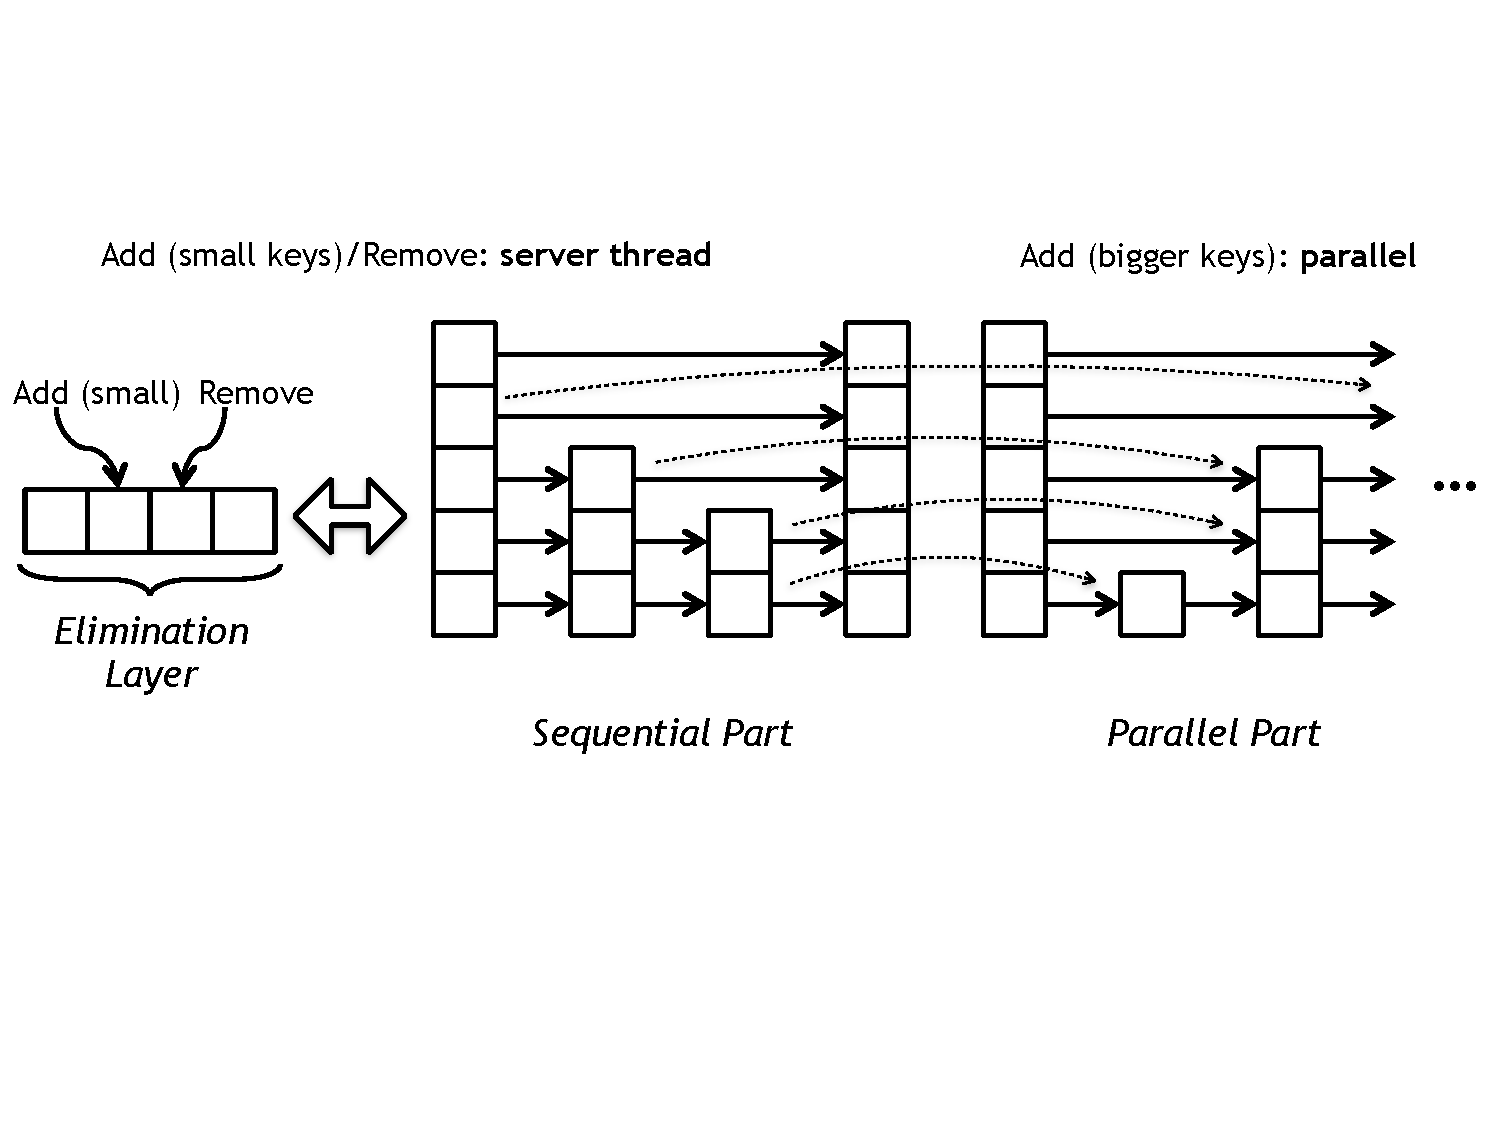
\includegraphics[width=0.9\textwidth]{graphics/pqe.pdf}
	\caption{Skiplist design \cite{calciu_adaptive_2014}.}
	\label{fig:pqe}
\end{figure}

\paragraph{Add()}

A thread executing \texttt{add($v$)} on the priority queue decides to insert the element concurrently into the parallel part if $v > \texttt{lastseq.key}$. Otherwise, the element is put into the elimination array as and add request. If the element becomes eligible for elimination ($v < \texttt{minValue}$) the operation can eliminate with any \texttt{removeMin()} occurring, otherwise the operation will be executed by the server thread \cite{calciu_adaptive_2014}.

\paragraph{RemoveMin()}

operations try to eliminate with an \texttt{add()} operation from the elimination array. If no operation is available, the thread writes a remove request to the array. It then gets either eliminated by a suitable \texttt{add()} operation or served by the server thread \cite{calciu_adaptive_2014}.

\subsection{Elimination and Combining}

Elimination allows operations to cancel each other out without accessing the shared datastructure. This reduces contention on the priority queue itself and therefore increases parallelism and scalability. The priority queue allows \texttt{removeMin()} operations to eliminate \texttt{add()} operations with keys smaller than \texttt{minValue} and vice versa. An array with a fixed size is used to store data the operations need to exchange \cite{calciu_adaptive_2014}.

\subsubsection{Elimination Array}

64 bit array slots are used to store a 32-bit value or one of the predefined opcodes as well as a unique stamp for every operation. Valid opcodes are: \texttt{EMPTY}, \texttt{REMREQ}, \texttt{INPROG}, and \texttt{TAKEN}. The values corresponding to these opcodes are not allowed to be used as values in the priority queue. These opcodes have following meaning:

\begin{description}
	\item[EMPTY] signals an unused slot of the elimination array.
	\item[REMREQ] is used by threads during a \texttt{removeMin()} operation to signal other threads the possibility to eliminate or instruct the server thread to remove an item from the priority queue.
	\item[INPROG] signals an adding thread that the server thread started to process the value that it wanted to add.
	\item[TAKEN] signals an adding thread that the value has been processed either by the server thread or a removing thread.
\end{description}

Other values stored in the elimination array are actual values being exchanged. The unique stamp also stored with the opcode/value is used for recognizing changes to the values stored in the elimination array and therefore ensuring linearizablity which will be covered in detail in section~\ref{sec:linearizablity}. This stamp is obtained by the thread ID and a thread-local operation counter \cite{calciu_adaptive_2014}.

\subsubsection{Operations and Elimination}

State transitions in the elimination array follow the state machine shown in figure~\ref{fig:combining-state}. Every slot is initially \texttt{EMPTY} with a stamp of 0. 

\begin{figure}[htb]
	\centering
	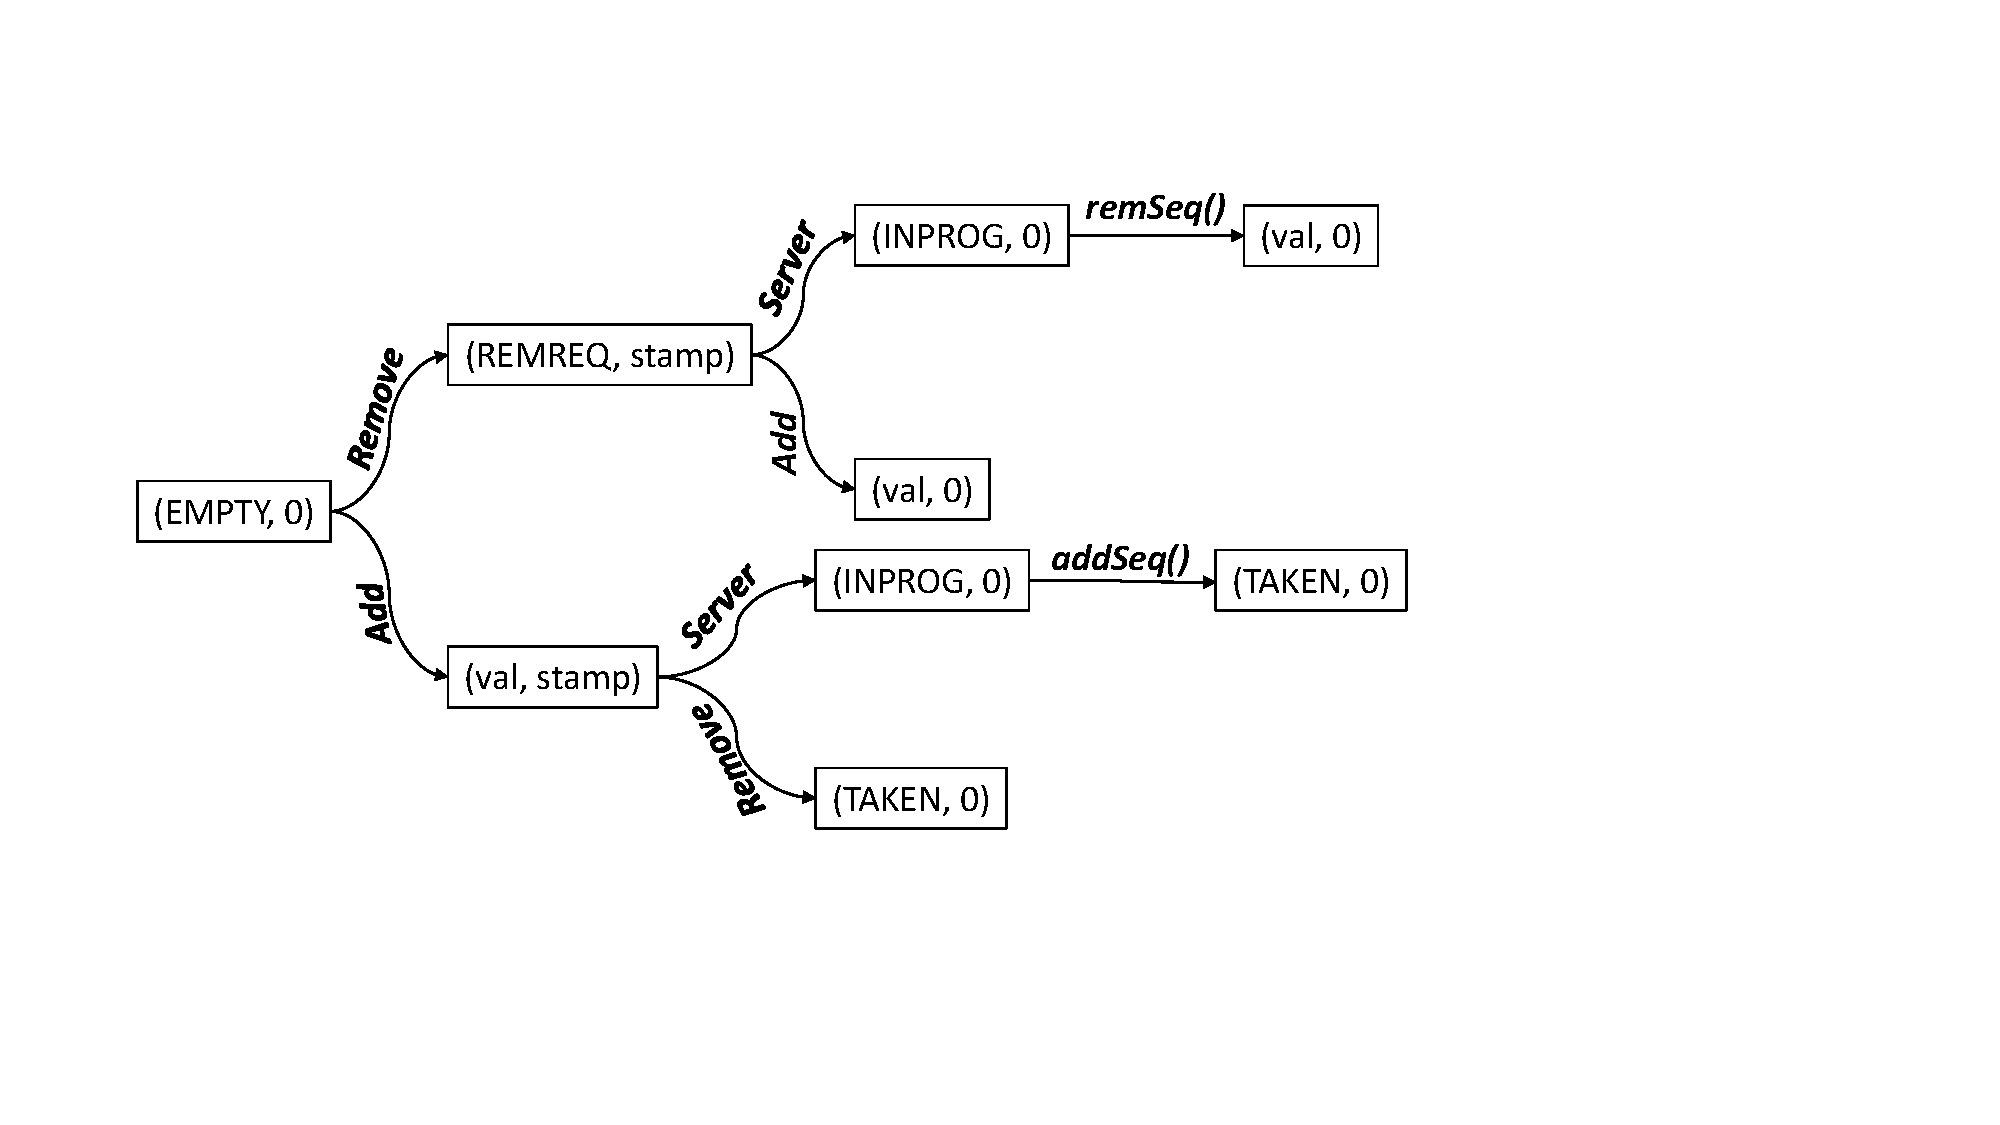
\includegraphics[width=0.9\textwidth]{graphics/combining-state.pdf}
	\caption{Elimination array state transitions \cite{calciu_adaptive_2014}.}
	\label{fig:combining-state}
\end{figure}

\paragraph{Add()} A thread trying to add a \texttt{key} (where $\texttt{key} < \texttt{minValue}$) iterates through all slots of the elimination array to find a \texttt{REMREQ} opcode. If it finds one and additionally $\texttt{key} < \texttt{minValue}$, the tread uses \texttt{CAS} to write its value including a stamp into this slot. If multiple attempts fail, the thread instead writes its value into a slot marked as \texttt{EMPTY} and waits for another or the server thread to use the value and change the opcode to \texttt{TAKEN}. The code for this operation can be found in the appendix in algorithm~\ref{alg:add} \cite{calciu_adaptive_2014}.

\paragraph{RemoveMin()} A thread removing an element from the priority queue iterates through the elimination array until it finds a value or an \texttt{EMPTY} slot in the elimination array. If the stamp of this value is greater than zero, it is checked whether the value is smaller than \texttt{minValue}, otherwise a non positive stamp indicates a value to respond to another \texttt{REMREQ}. In the case of the value being a current minimum of the priority queue the thread uses \texttt{CAS} to replace the value with \texttt{TAKEN}. In the case of finding an empty slot first, a \texttt{REMREQ} with a unique stamp is posted to this slot. Then the thread waits for another thread to eliminate this remove request or the server thread to actually remove one element from the priority queue and post it to this slot of the elimination array. The code for this operation can be found in the appendix in algorithm~\ref{alg:removeMin} \cite{calciu_adaptive_2014}.

\paragraph{Server Thread} The dedicated server thread is implemented to ensure progress of all threads as not all remove requests and add operations eliminate. The server thread collects all add and remove requests and executes them sequentially on the sequential part of the skiplist. To keep the implementation linearizable the server thread first swaps the value or remove request with \texttt{INPROG}. After the insertion \texttt{TAKEN} is written to the according slot, for removes the value with stamp 0 is written to the slot. The code for this operation can be found in the appendix in algorithm~\ref{alg:Execute} \cite{calciu_adaptive_2014}.

\subsection{Skiplist Operations}

The priority queue operations \texttt{add()} and \texttt{removeMin()} use the operations described in this section to manipulate the skiplist.

\subsubsection{Sequential Part}

The \texttt{addSeq()} and \texttt{removeSeq()} operations are just straight forward skiplist operations as they do not have to deals with any synchronization mechanism. The code for \texttt{removeSeq()} is shown in algorithm~\ref{alg:RemoveSeq} \cite{calciu_adaptive_2014}.

\subsubsection{Parallel Part addPar()}

The \texttt{addPar()} operation relies on a Single-Writer-Multi-Reader lock to not manipulate any pointers while head-moving operation are running. To keep the critical section as short as possible this operation first performs a \texttt{cleanFind()} as seen in algorithm~\ref{alg:CleanFind}. It searches for the position to insert the element, then acquires the read lock, and checks a timestamp variable manipulated through locking. If the checked timestamp changed between the successful \texttt{find()} and the check within the critical section the operation has to retry from the start. The code is shown in algorithm~\ref{alg:AddPar} \cite{calciu_adaptive_2014}.

\subsubsection{Head-Moving Operations}

The head-moving operations are responsible for moving the boundary between the sequential and the parallel part of the skiplist. At the beginning of such a operation a write-lock is acquired to keep other threads from adding elements in parallel while the boundary is manipulated.

\paragraph{moveHead()}

The \texttt{moveHead()} operation is used to extract a new sequential part from the skiplist if a remove request cannot be served because of an empty sequential part. At first the algorithm decides on how many elements should be moved to the sequential part. The number changes adaptive between $2^3$ and $2^{16}$. If more than $N$ insertions were performed in the sequential part since the last \texttt{moveHead()} was performed, the number of elements to move is doubled, if less than $M$ are inserted then the number is halved. The code is shown in algorithm~\ref{alg:MoveHead} \cite{calciu_adaptive_2014}.

\paragraph{chopHead()}

The \texttt{chopHead()} operation is called if no remove operations have been performed in a while. This operation relinks the sequential and the parallel part to form a fully parallel skiplist. The code is shown in algorithm~\ref{alg:ChopHead} \cite{calciu_adaptive_2014}.

\subsection{Hardware Transactions}

\subsubsection{Head-Moving Operations}

\subsubsection{addPar()}

% !TEX root = ../paper.tex

\section{Linearizablity}
\label{sec:linearizablity}

Linearizability as defined by \citeauthor{herlihy_linearizability:_1990} is a widely used correctness condition for concurrent objects. Linearizability guarantees that each operation appears to have an atomic effect at some point between its invocation and response. This point is typically referred to as linearization point. Combinations of linearizable operations are still linearizable which leads to the definition of a linearizable object. An object is linearizable, if each sequence of operations on this object is linearizable \cite{herlihy_linearizability:_1990}.

For the priority queue to meet the desirable linearizability condition it remains to show that each operation is linearizable. 

\subsection{Skiplist Operations}

\paragraph{AddPar() and AddSeq()}

both have their linearization point at the moment the element is added to the bottom level of the skiplist. The only exception is the insertion of a value that is smaller than \texttt{minValue}. In this case the \texttt{minValue} has to be updated. If there is a sequential part, this is done by the server thread, otherwise the performing thread retries until it succeeds or another thread updates it to an even smaller value  \cite{calciu_adaptive_2014}.


\paragraph{MoveHead() and ChopHead()}

both execute while holding the write lock, which means they execute without any thread interfering as no \texttt{addPar()} operation is allowed to run and the other sequential operations are only invoked by the server thread itself. These operations linearize when the lock is released \cite{calciu_adaptive_2014}.

\subsection{Elimination and Combining}

The unique stamps introduced in section~\ref{sec:eliminationArray} are necessary to avoid the ABA\footnote{\enquote{ABA is not an acronym and is a shortcut for stating that a value at a shared location can change from A to B and then back to A} \cite[185]{dechev_understanding_2010}.} problem. Without this stamp a thread performing an elimination could be interrupted by other threads using the same slot without him noticing it. This would result in an exchange of values with another thread than anticipated, which would break linearizability.

Figure~\ref{fig:correctness_elim} visualizes at which point in time two threads involved in an elimination linearize. A thread either inserting or removing a value has to check the exchanged value for being smaller than \texttt{minValue}. In that case the linearization point is at the time of this observation. Other interleaving operations could manipulate the \texttt{minValue} after this observation without breaking linearizability.

\begin{figure}
	\centering
	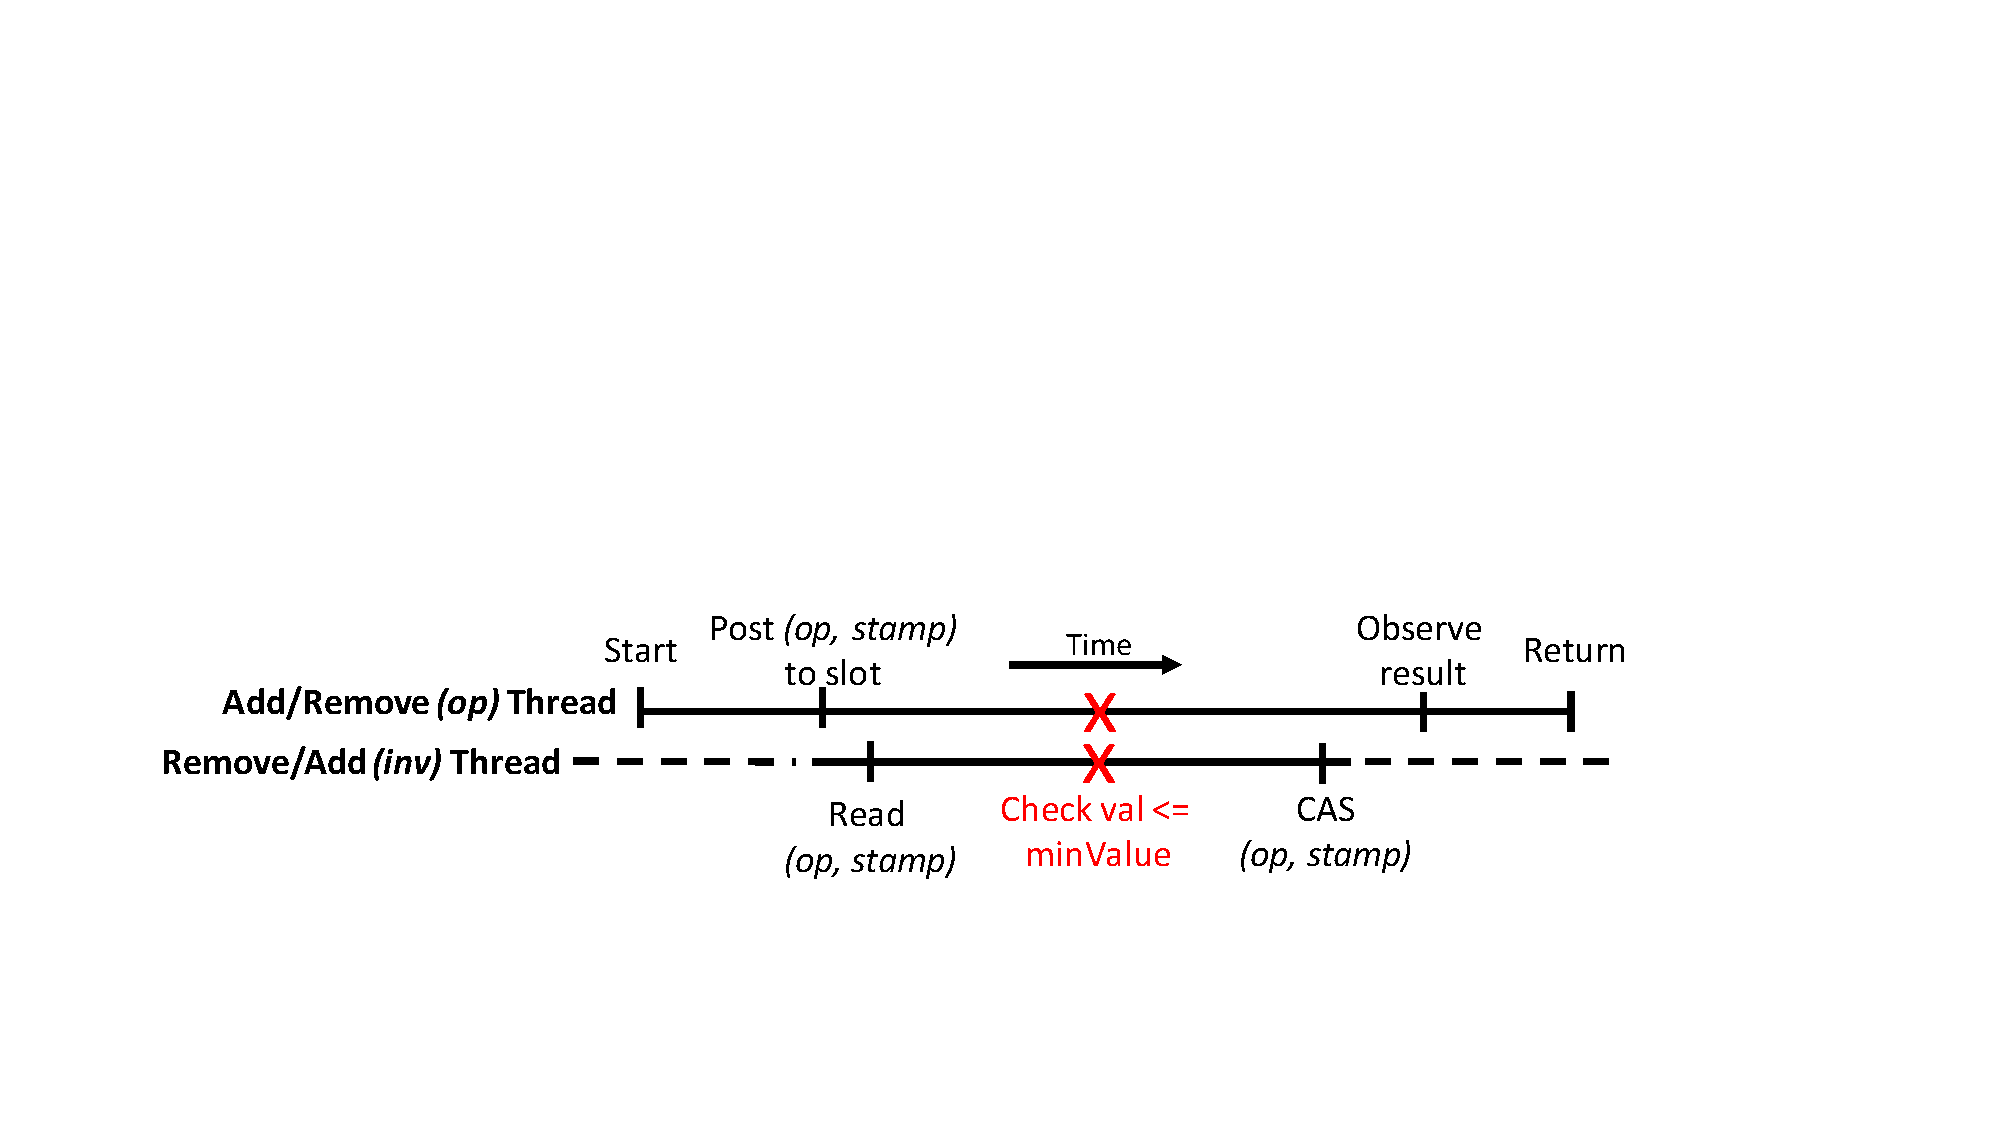
\includegraphics[width=0.9\textwidth]{graphics/correctness2.pdf}
	\caption{Execution of an \emph{op} thread and an \emph{inv} thread eliminating each other's operation. The linearization point is determined through the observation of the exchanged value being smaller than \texttt{minValue}. It is marked with a red X \cite{calciu_adaptive_2014}.}
	\label{fig:correctness_elim}
\end{figure}

Figure~\ref{fig:correctness_server} shows the point in time a thread linearizes while exchanging values with the server thread. The linearizability follows from the linearizability of the skiplist itself and the sequential execution on the skiplist \cite{calciu_adaptive_2014}. 

\begin{figure}[htb]
	\centering
	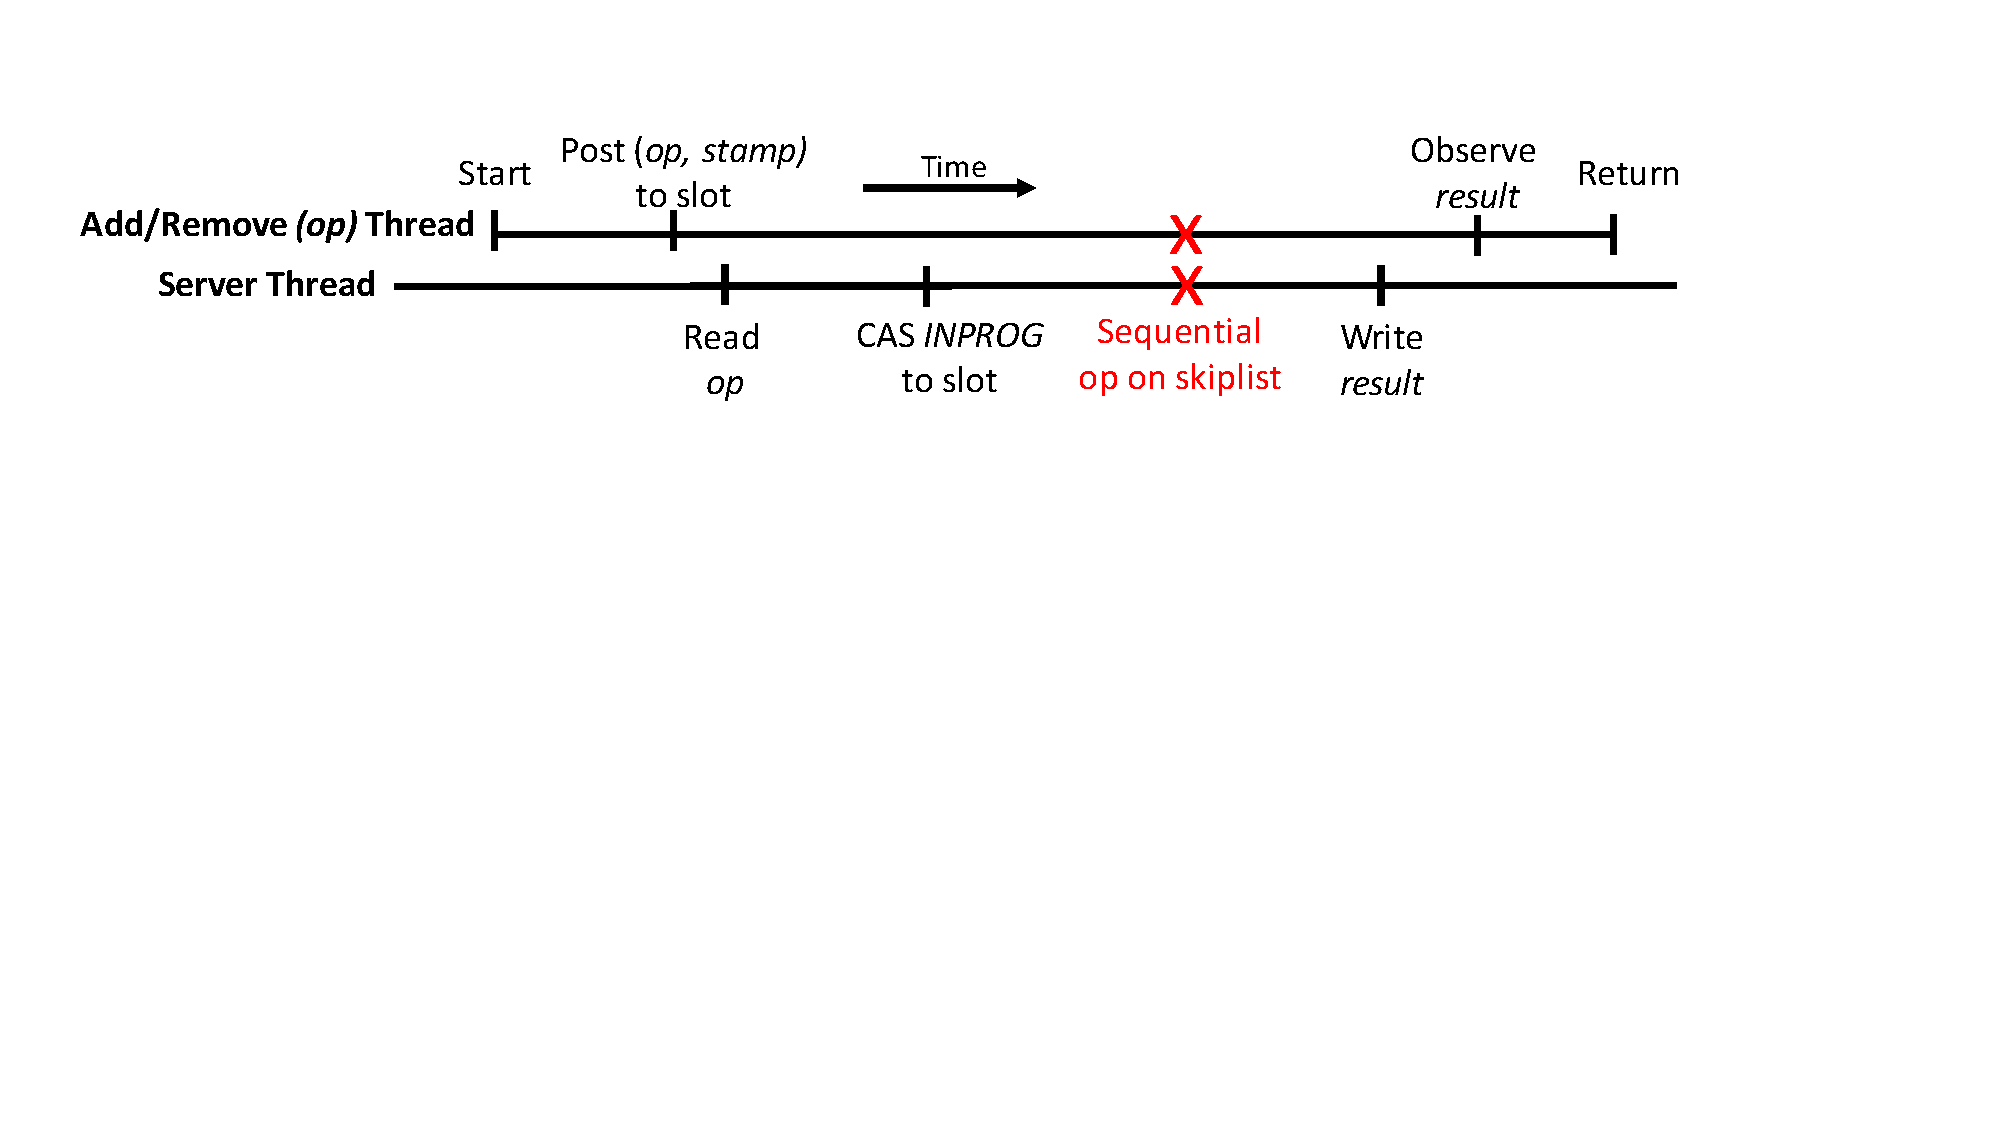
\includegraphics[width=0.9\textwidth]{graphics/correctness1.pdf}
	\caption{Execution of an \emph{op} having its operation served by the server thread. The linearization point is determined through the sequential operating server thread and is marked with a red X \cite{calciu_adaptive_2014}.}
	\label{fig:correctness_server}
\end{figure}

\subsection{Hardware Transactions}

When using transactions the linearization points are straight forward to determine. Each operation linearizes when the transaction completes successfully. 
% !TEX root = ../paper.tex

\section{Evaluation}

This section describes the result of both described algorithms. Although the   Newer priority queue implementation According to later published papers like \cite{braginsky_cbpq:_2016, } the performa



\subsection{Single-Writer-Multi-Reader Lock Implementation}

\subsubsection{Head-Moving Operations Overhead}

\subsection{Hardware Transactional Memory Implementation}

\subsubsection{Aborted Transaction Overhead}

\subsection{Comparison with succeeding papers}

C++ and compiled with a -O3 optimization level

\cite{braginsky_cbpq:_2016, } way better (used original code of this paper)

algorithm doesn't seem to scale much on multi socket machine, significant performance drop after useage of

AMD Opteron (TM) 6272
16-core processors, overall 64 threads. The machine was operated by Linux OS
(Ubuntu 14.04)
\subsection{Evaluating the Overhead of \texttt{PQ::moveHead()} and \texttt{PQ::chopHead()}}
\label{Sec-Eval-Move}

Maintaining separate skiplists for the sequential and the parallel part of the priority queue is beneficial for the overall throughput, but adds some overhead, which we quantify in this section. 
The number of elements that become part of the sequential skiplist changes dynamically based on the observed mix of operations. This adaptive behavior helps reduce the number of \texttt{moveHead()} and \texttt{chopHead()} operations required.  
Table~\ref{fig:sparc_headmove} shows the percentage of the number of head-moving operations out of the total number of \texttt{PQ::removeMin()} operations for different mixes of \texttt{PQ::add()} and \texttt{PQ::removeMin()} operations. The head-moving operations are rarely called due to the priority queue's adaptive behavior. 

\begin{table}[htb]
  \centering
	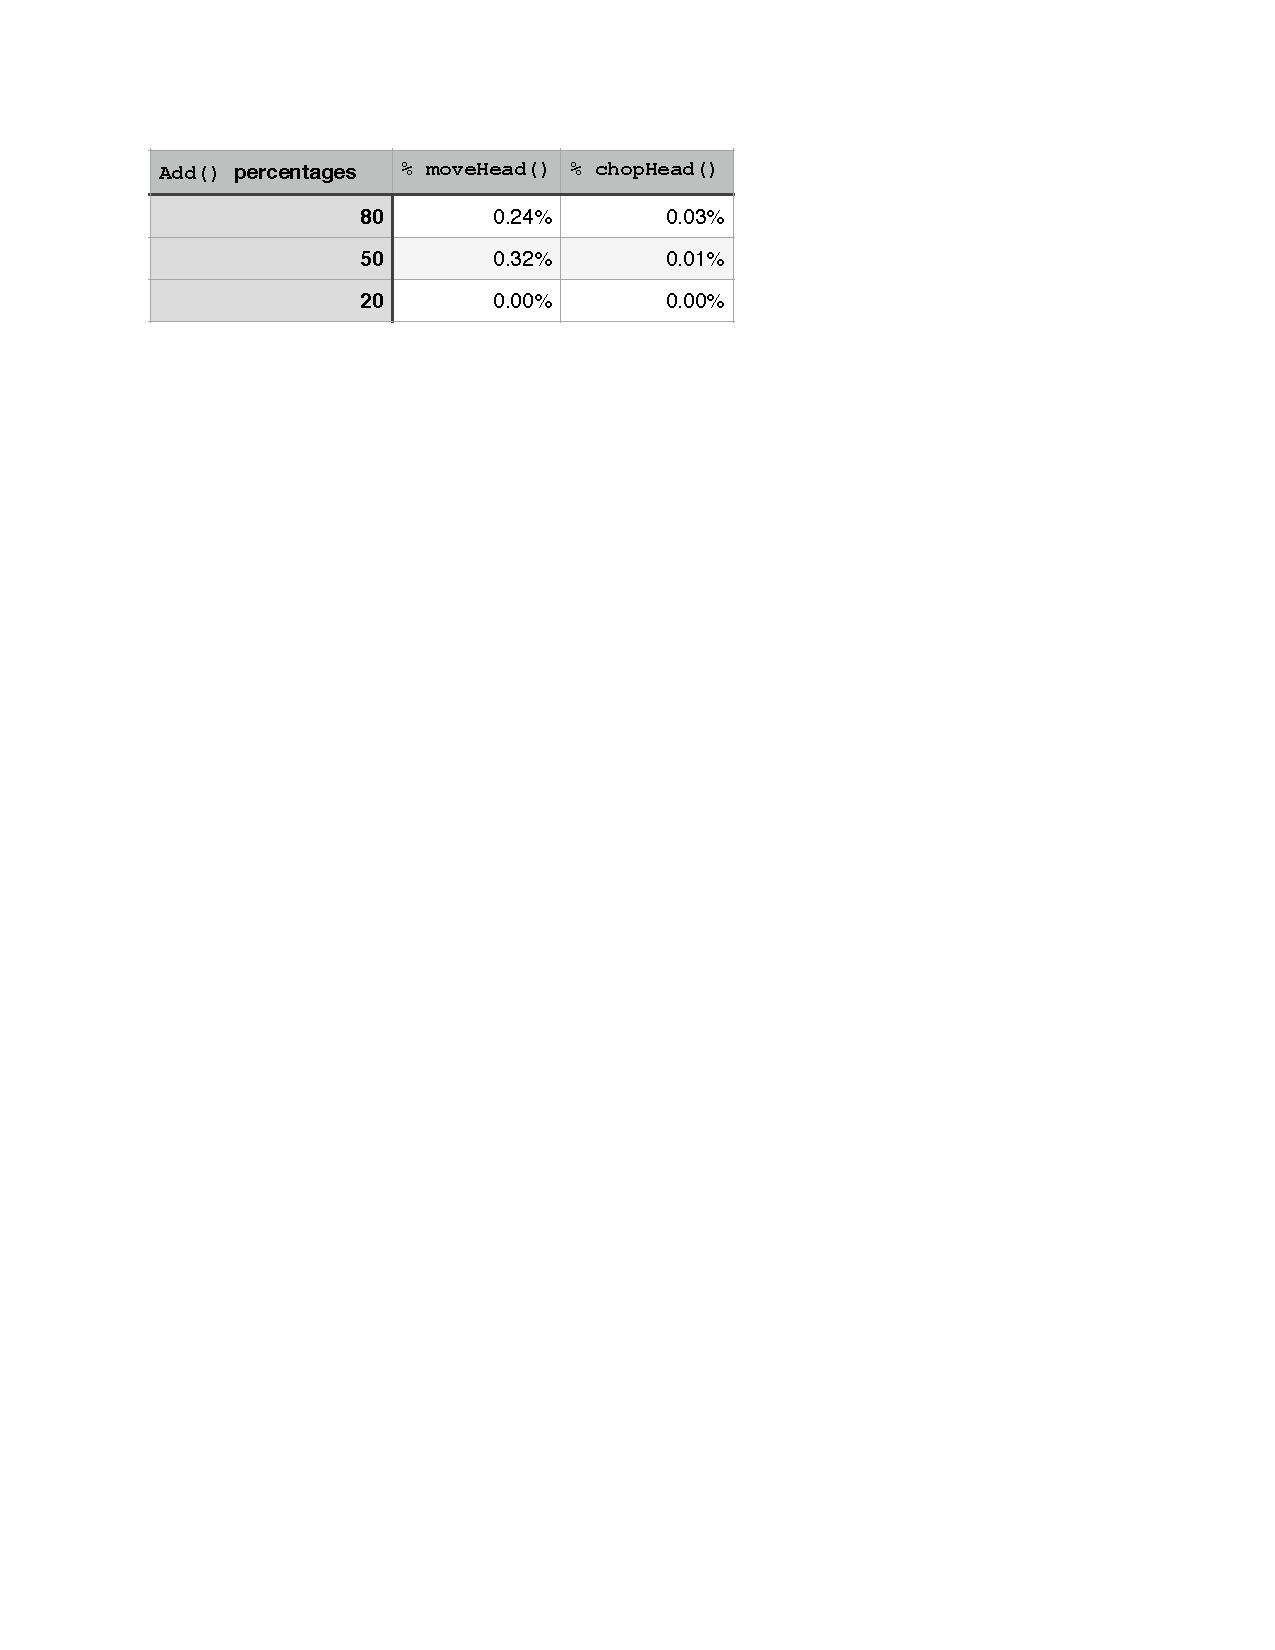
\includegraphics[width=0.65\textwidth]{img/sparc-stats-headmove.pdf}
	\caption{The number of head-moving operations as a percentage of the total number of \texttt{PQ::removeMin()} operations, considering different \texttt{add()} and \texttt{removeMin()} mixes.}
\label{fig:sparc_headmove}
\end{table}


\section{Hardware Transactions}
\label{Sec-HardwareTransactions}

%Designing concurrent data structures involves complicated synchronization between threads, often implemented using CAS instructions. Certain design decisions circumvent the limitation that we cannot change or check multiple locations atomically. For example, our priority queue design packs a value and a stamp together in order to check both in the same CAS operation, as explained in section~\ref{Sec-Design-Elimination}. Also, we have to use an extra value in the elimination array, INPROG, to mark an element that is being added or removed by the server thread. Finally, the design of the underlying skiplist is complicated by the need to synchronize parallel adds with the \texttt{moveHead()} operation. 

Transactional memory~\cite{Herlihy:1993:TMA:173682.165164} is an optimistic mechanism to synchronize threads accessing shared data. Threads are allowed to execute critical sections speculatively in parallel, but, if there is a data conflict, one of them has to roll back and retry its critical section. Recently, IBM and Intel added HTM instructions to their processors~\cite{wang:2012:pact,haswell:2012:rtm}. 
In our priority queue implementation, we used Intel's Transactional Synchronization Extensions (TSX)~\cite{haswell:2012:rtm} to simplify the implementation and reduce the overhead caused by the synchronization necessary to manage a sequential and a parallel skiplist. 
%In this section, we discuss the necessary changes, adequacy, and results of using TSX to simplify and improve performance of our priority queue. 
We evaluate our results on an Intel Haswell four core processor, Core i7-4770, with hardware transactions enabled (restricted transactional memory - RTM), running at 3.4GHz. There are 8GB of RAM shared across the machine and each core has a 32KB L1 cache. Hyperthreading was enabled on our machine so we collected results using all 8 hardware threads. Hyperthreading causes resource sharing between the hyperthreads, including L1 cache sharing, when running with more than 4 threads, thus it can negatively impact results, especially for hardware transactions. We did not notice a hyperthreading effect in our experiments. We used the GCC 4.8 compiler with support for RTM and optimizations enabled (-O3).  

\subsection{Skiplist}
\label{Sec-Transactions-SkipList}

The Single-Writer-Multi-Readers lock used to synchronize the sequential and the parallel skiplists complicates the priority queue design and adds overhead. In this section, we explore an alternative design using hardware transactions. 
However, the naive approach of making all operations transactional causes too many aborts. Instead, the server increments a timestamp whenever a head-moving operation - \texttt{SL::moveHead()} or \texttt{SL::chopHead()} - starts or finishes. A \texttt{SL::addPar()} operation first reads the timestamp and executes a nontransactional \texttt{SL::find()} and then starts a transaction for the actual insertion, adding the server's timestamp to its read set and aborting if it is different from the initially recorded value. Moreover, if the timestamp changes after starting the transaction, indicating a head-moving operation, the transaction will be aborted due to the timestamp conflict.  
If the timestamp is valid, \texttt{SL::find()} must have recorded the predecessors and successors of the new bucket at each level $i$ in \texttt{preds[i]} and \texttt{succs[i]}, respectively. If a bucket already exists, the counter is incremented inside the transaction and the operation completes. If the bucket doesn't exist, the operation proceeds to check if \texttt{preds[i]} points to \texttt{succs[i]} for all levels $0 \le i \le \maxLvl$. If so, the pointers have not changed before starting the transaction and the new bucket can be correctly inserted between \texttt{preds[i]} and \texttt{succs[i]}. Otherwise, we commit the (innocuous) transaction, yet restart the operation.


%%%%%%%%%%%%%%%%%%%%%%%%5

%In the \texttt{SL::addPar()} operation, we initially tried to include our \texttt{SL::find()} inside a transaction, together with the \emph{mutable} operations, those that perform pointer changes or that increment counters. However, we were having too many aborts caused by a poor interaction of mutable interactions and the finds. We finally decided to use an approach similar to the one in the lock-based implementation: our \texttt{SL::find()} first executes outside a transaction, and then \texttt{SL::addPar()} starts a transaction. The function proceeds to check a timestamp indicating whether a head-moving operation took place.

%If the timestamp is valid, \texttt{SL::find()} returned the predecessor and successor of the newly inserting bucket at each level $i$ in \texttt{preds[i]} and \texttt{succs[i]}, respectively. If a bucket is found, the counter is incremented inside the transaction and the operation finishes. Otherwise, the operation proceeds to check if \texttt{preds[i]} points to \texttt{succs[i]} for all levels $0 \le i \le \maxLvl$. If that happens, indicating that the pointers did not change before acquiring the transaction, the new bucket is inserted between \texttt{preds[i]} and \texttt{succs[i]} for all levels $0 \le i \le \maxLvl$. In the negative case, we commit the (innocuous) transaction, yet restart the operation.

%The head-moving operations (\texttt{SL::moveHead()} and \texttt{SL::chopHead()}) increment the timestamp when they start executing and when they finish executing. 
%This way, they are able to interrupt inserting \texttt{SL::addPar()}s in the parallel part in a very natural manner: when the timestamp associated with these operations moves, the transactions are immediately aborted as the timestamp is in their read set.

%%%%%%%%%%%%%%%%

Figures~\ref{fig:tsx1} and~\ref{fig:tsx2} compare the performance of the lock-based implementation and the implementation based on hardware transactions for two different percentages of \texttt{PQ::add()}s and \texttt{PQ::removeMin()}s. When fewer \texttt{PQ::removeMin()} operations are present, the timestamp changes less frequently and the \texttt{PQ::add()} transactions are aborted fewer times, which increases performance  in the 80\%-20\% insertion-removal mix. In the $50\%$-$50\%$ mix, we obtain results comparable to the \emph{pqe} algorithm using the lock-based approach, albeit with a much simpler implementation.

\begin{figure}[htb]
\centering
\begin{minipage}{.495\textwidth}
	\centering
  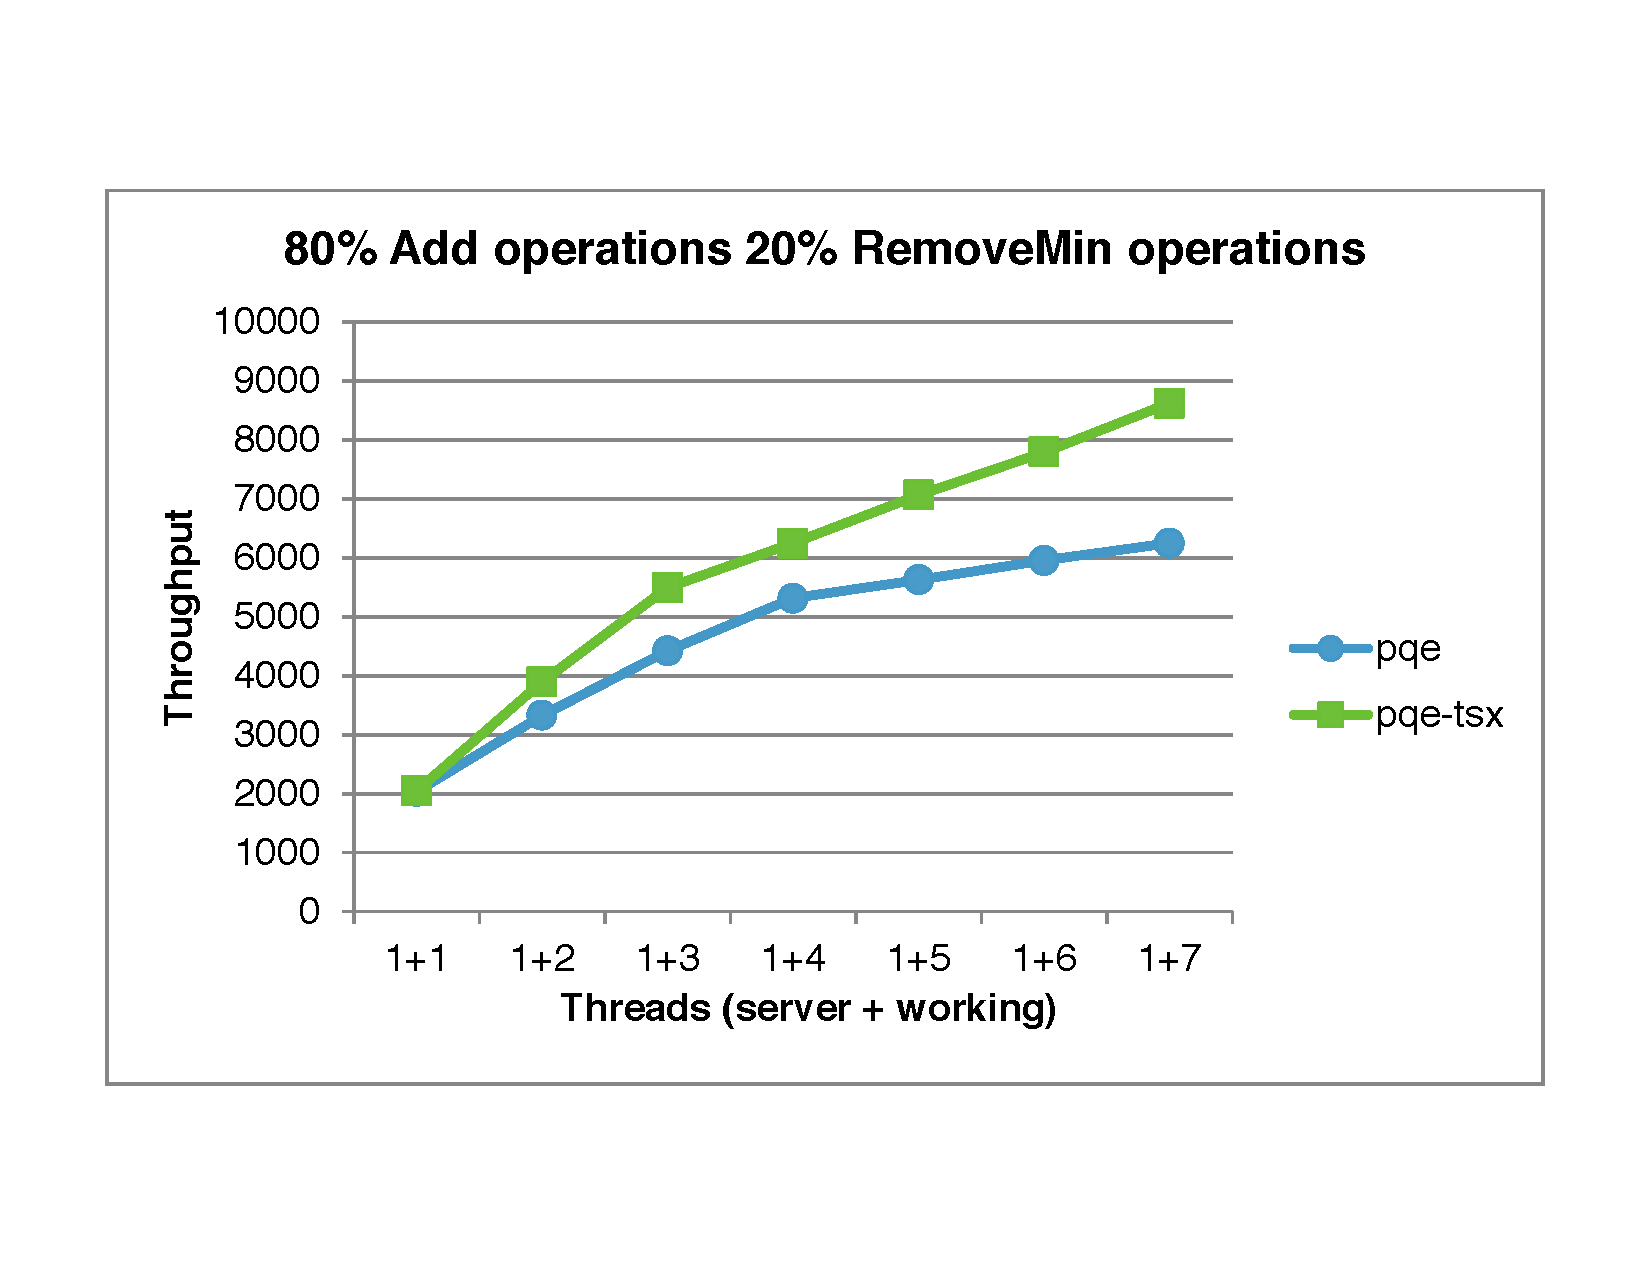
\includegraphics[width=\linewidth]{img/tsx-80-20.pdf}
\caption{Priority queue performance when we use a transaction-based dual skiplist; 80\% \texttt{add()}s, 20\% \texttt{removeMin()}s.}
\label{fig:tsx1}
\end{minipage}%
\hfill%
\begin{minipage}{.495\textwidth}
	\centering
  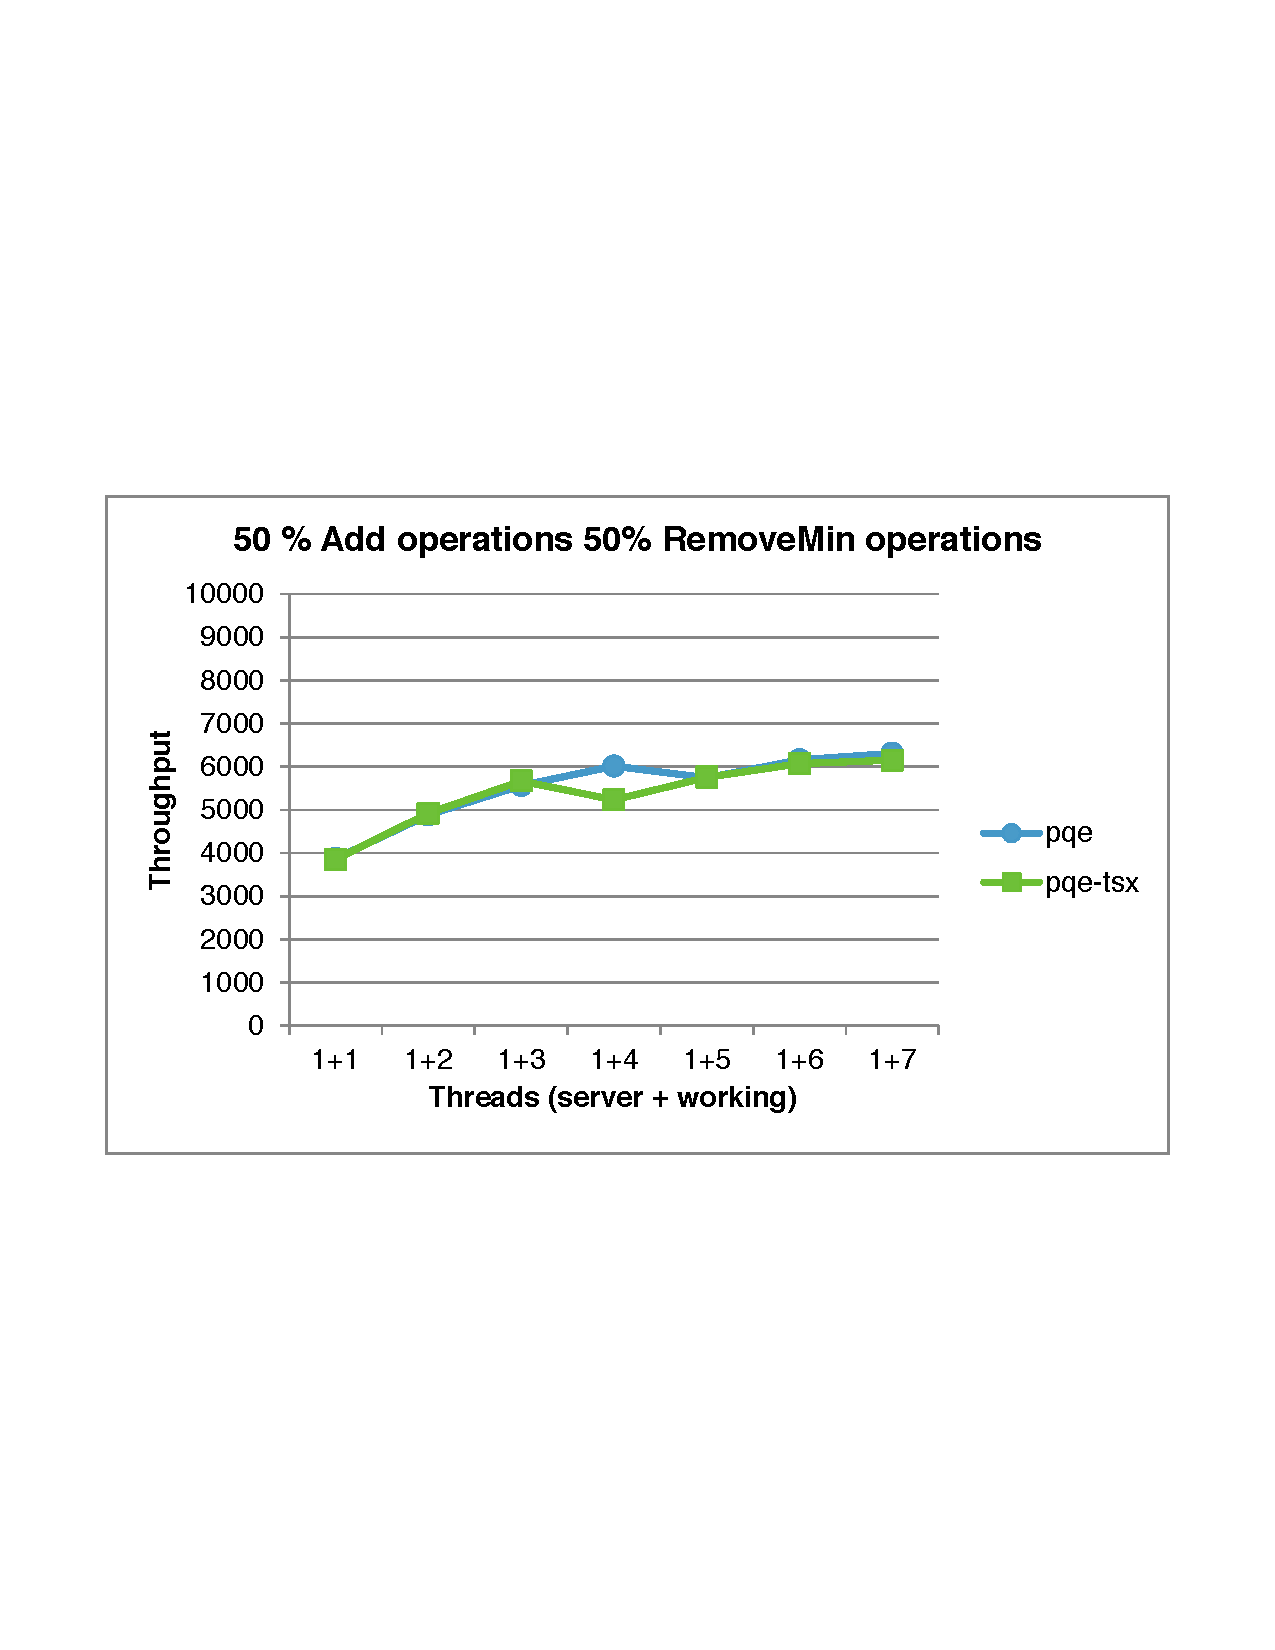
\includegraphics[width=\linewidth]{img/tsx-50-50.pdf}
\caption{Priority queue performance when we use a transaction-based dual skiplist; 50\% \texttt{add()}s, 50\% \texttt{removeMin()}s.}
\label{fig:tsx2}
\end{minipage}
\end{figure}

\subsection{Evaluating the Overhead of Aborted Transactions}
\label{Sec-Eval-Aborted}

The impact of aborted transactions is reported in Tables~\ref{tbl:tsx-stat1} and~\ref{tbl:tsx-stat2}. As the number of threads increases, the number of transactions per successful operation 
also increases, as does the percentage of operations that need more than 10 retries to succeed. 
Note that the innocuous transactions that find inconsistent pointers, changed between the \texttt{SL::find()} and the start of the transaction are not included in the measurement. 
After 10 retries, threads give up on retrying the transactional path and the server executes the operations on their behalf, either in the sequential part, using sequential operations, or in the parallel part, using \texttt{CAS()} for the pointer changes,  but without holding the readers lock. The server does not need to acquire the readers lock because no other thread will try to acquire the writer lock. 


\begin{table}[htb]
\centering
\begin{minipage}{.49\textwidth}
	\centering
  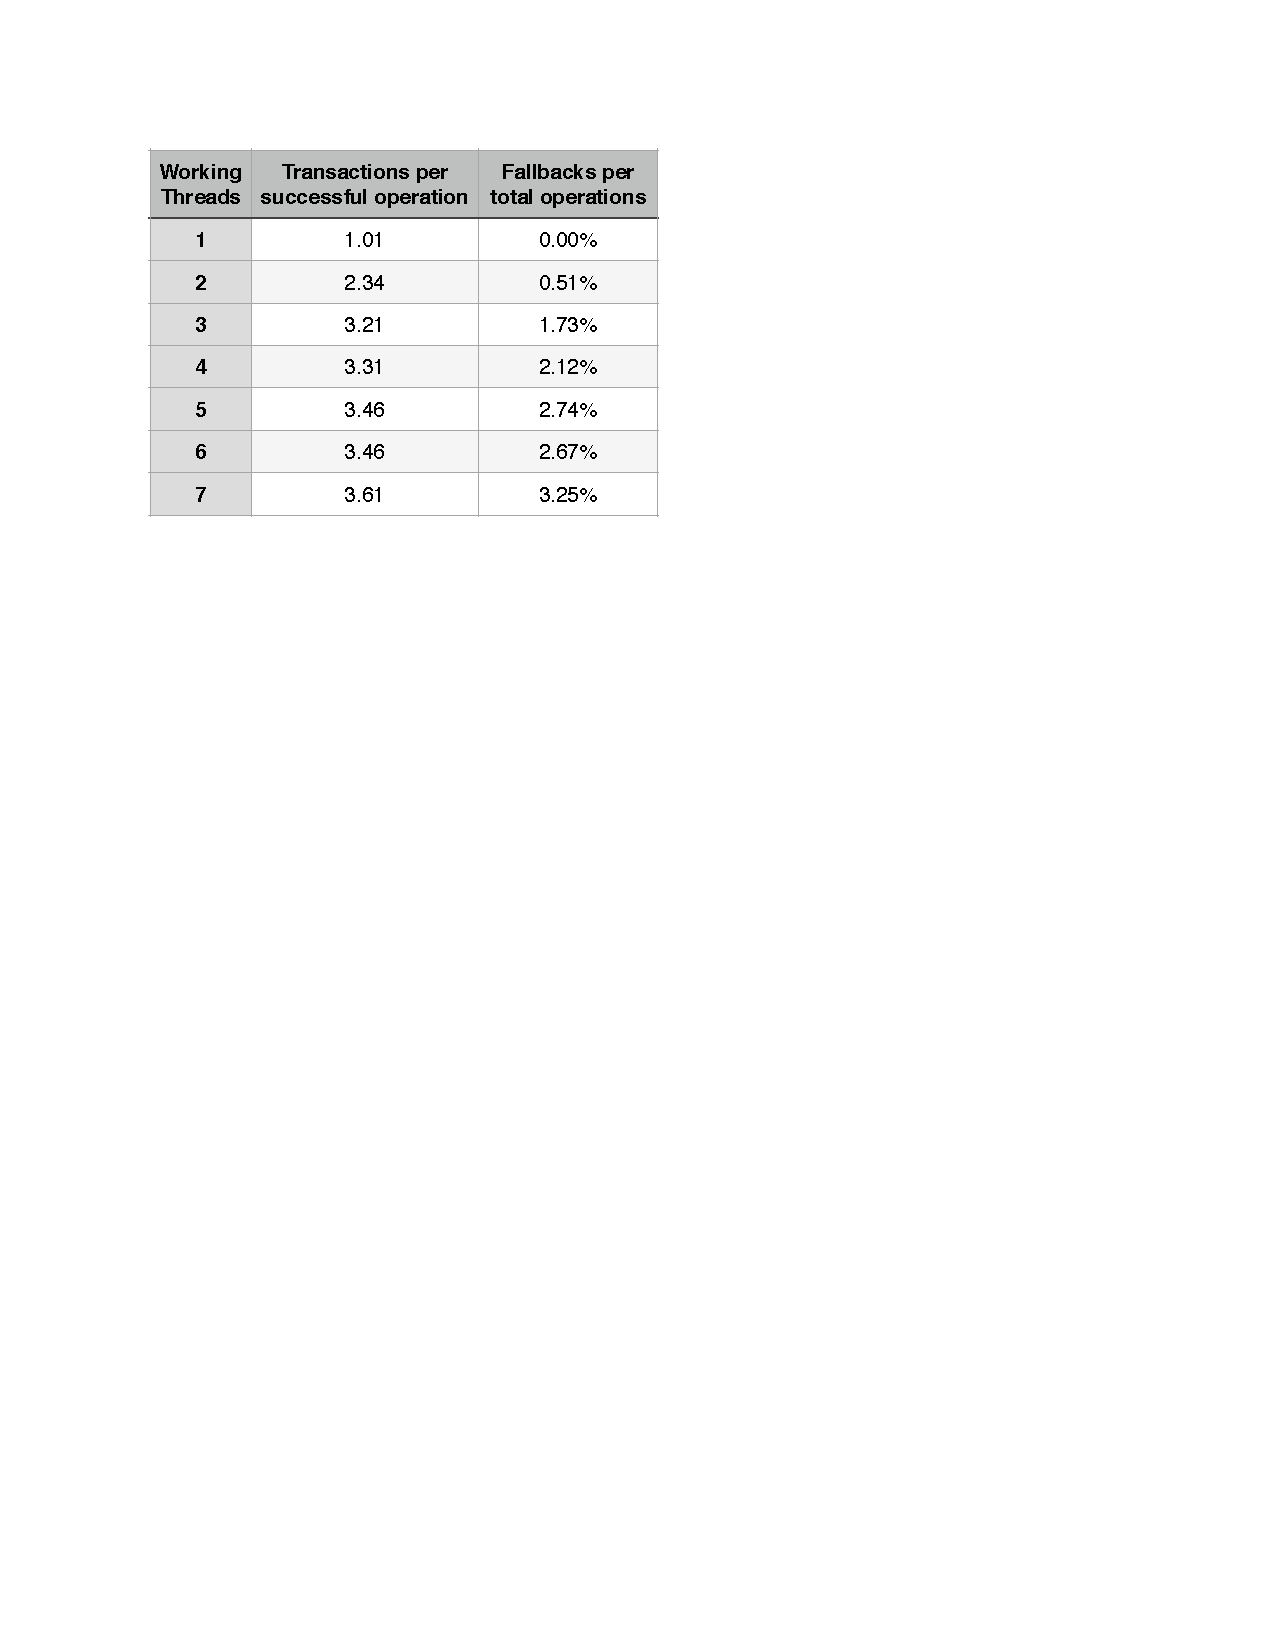
\includegraphics[width=\linewidth]{img/tsx-stat-threads.pdf}
\caption{Transaction stats for varying \# of threads, with 50\% \texttt{PQ::add()}s and 50\% \texttt{PQ::removeMin()}s}
\label{tbl:tsx-stat1}
\end{minipage}%
\hfill%
\begin{minipage}{.49\textwidth}
	\centering
  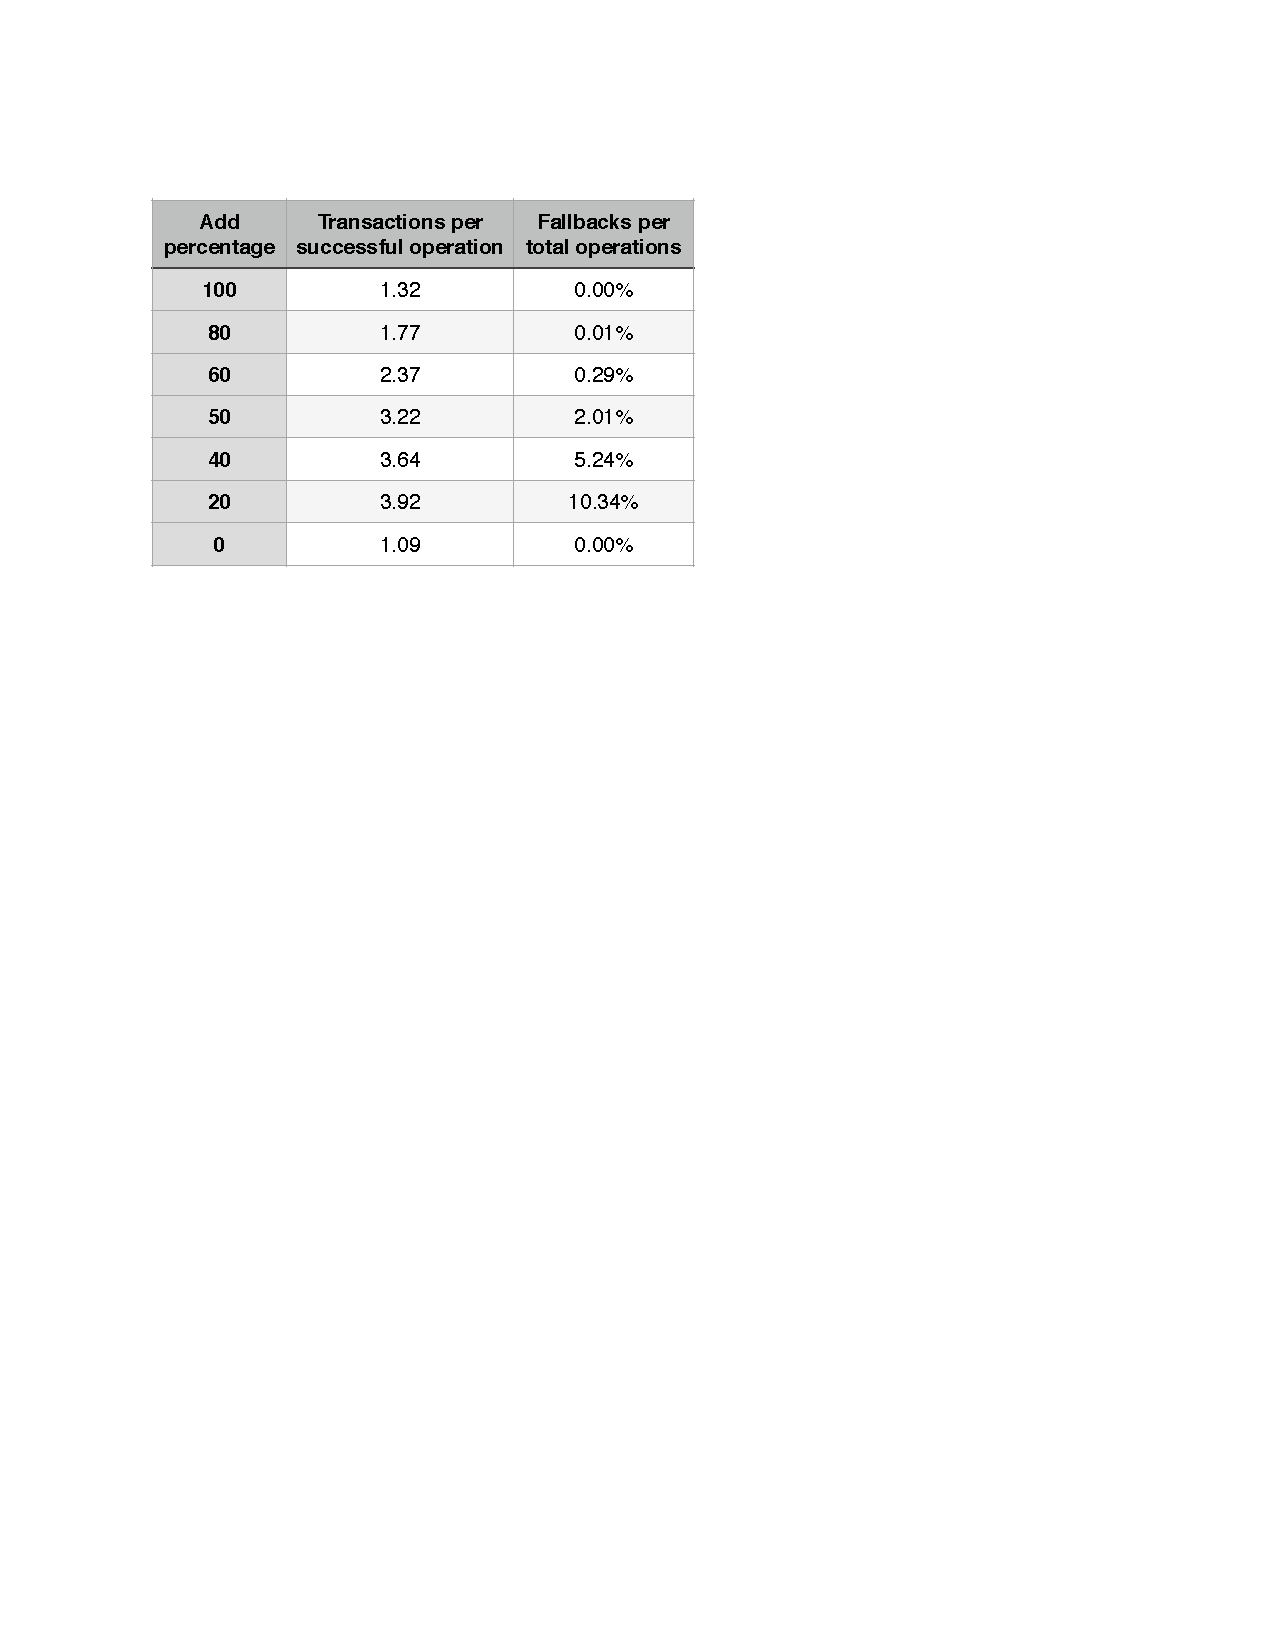
\includegraphics[width=\linewidth]{img/tsx-stat-percents.pdf}
\caption{Transaction stats for varying mixes, with 1 server thread and 3 working threads.}
\label{tbl:tsx-stat2}
\end{minipage}
\caption{Statistics on the overhead of aborted transactions.}
\end{table}

The number of transactions per successful operation is at most $3.92$, but $3.22$ in the $50\%-50\%$ case. The percentage of operations that get executed by the server (after aborting 10 times) is at most $10\%$ of the total number of operations, but between $1.73\%$ and $2.01\%$ for the $50\%-50\%$ case.

% !TEX root = ../paper.tex

\section{Conclusion}

\todo{We summarize the contribution of the papers and this seminar paper.}

\bibliography{pqe_disc_14}
\bibliographystyle{plain}

\newpage
\appendix

\section{Algorithms for the Concurrent Skiplist}
\label{App-Algorithms-ConcurrentSkiplist}

In this section, we present the algorithms for the concurrent skiplist described in Sec.~\ref{Sec-Design-ConcurrentSkiplist}. The skiplist contains a Single-Writer-Multi-Readers lock with writer preference, called simply \texttt{lock}. In terms of notation, \texttt{lock.acquireR()} acquires the lock for reads, and \texttt{lock.acquireW()} acquires the lock for writes. The \texttt{SL::removeSeq()} skiplist procedure is described in Alg.~\ref{Alg-RemoveSeq}.

\begin{algorithm}[!htb]
\caption{SL::removeSeq()}
\label{Alg-RemoveSeq}
\begin{algorithmic}[1]
\If{minValue $=$ \maxInt}
	\State \Return \maxInt
\EndIf
\If{currSeq $=$ \nullvalue}
	\State moveHead()
\EndIf
\State key \attr currSeq.key
\State currSeq.counter \attr currSeq.counter - 1
\If{currSeq.counter $= 0$}
	\While{currSeq $\ne$ lastSeq}
		\State currSeq \attr currSeq.next[0]
		\If{currSeq.counter $> 0$}
			\State minValue = currSeq.key
			\State \Return key
		\EndIf
	\EndWhile
	\State moveHead()
\EndIf
\State \Return key
\end{algorithmic}
\end{algorithm}

The variable \texttt{lock.timestmap} contains the timestamp associated with the lock (and hence with the head-moving operations). Algorithm~\ref{Alg-CleanFind} returns a pair of elements $(b,r)$: $b$ is a bucket found using the skiplist \texttt{SL::find()} operation, and $r$ is a boolean defined as follows. If a head-moving operation happened anywhere between Lines~\ref{algFLT:checkstamp1} and~\ref{algFLT:checkstamp2}, the timestamp moved and $r$ will be false.

\begin{algorithm}[!htb]
\caption{cleanFind($v$, preds, succs)}
\label{Alg-CleanFind}
\begin{algorithmic}[1]
\State $t$ \attr lock.timestamp \label{algFLT:checkstamp1}
\State $b$ \attr find(headPar, $v$, preds, succs)
\State lock.acquireR()
\If{$t$ $<$ lock.timestamp} \label{algFLT:checkstamp2}
	\State lock.release()
	\State \Return $(\nullvalue, \mathbf{false})$
\EndIf
\State \Return $(b, \mathbf{true})$
\end{algorithmic}
\end{algorithm}

The \texttt{SL::addPar()} skiplist procedure is described in Alg.~\ref{Alg-AddPar}. It uses the clean find protocol above. It performs a clean find, followed by mutable operations (either increasing a counter or inserting a bucket), executed with \texttt{lock} acquired for reading.

\begin{algorithm}[!htb]
\caption{SL::addPar($v$)}
\label{Alg-AddPar}
\begin{algorithmic}[1]
\If{$v$ $\le$ lastSeq.key}
	\State \Return \textbf{false}
\EndIf
\State $(b,r)$ \attr cleanFind($v$, preds, succs) \label{algAddPar:find}
\If{$r$ = \textbf{false}}
	\State \textbf{restart} at line~\ref{algAddPar:find}
\EndIf
\If{$b \ne \nullvalue$} \label{algAddPar:incblock}
	\State Atomically increment $b$.counter
	\State lock.release()
	\State \Return \textbf{true}
\EndIf
\State $b$ \attr newNode($v$)
\For{$i$: 1 $\rightarrow$ $b$.topLevel}
	\State $b$.next[i] \attr succs[i]
\EndFor
\If{\textbf{not} CAS(preds[0].next[0]: succs[0] $\rightarrow$ $b$)}
	\State lock.release()
	\State \textbf{restart} at line~\ref{algAddPar:find}
\EndIf
\Repeat
	\State $m$ \attr minValue
\Until{$m \le v$ \textbf{or} CAS(minValue: $m \rightarrow v$)}
\For{$i$: 1 $\rightarrow$ $b$.topLevel}
	\State $b$.next[i] \attr succs[i]
	\If{CAS(preds[i].next[i]: succs[i] $\rightarrow$ $b$)}
		\State \Continue
	\EndIf
	\State lock.release()
	\Repeat
		\State $(b,r)$ \attr cleanFind($v$, preds, succs)
	\Until{$r = \mathbf{true}$}
	\If{$b = \nullvalue$}
		\State lock.release()
		\State \Return \textbf{true}
	\EndIf
\EndFor
\State \Return \textbf{true}
\end{algorithmic}
\end{algorithm}

The \texttt{SL::moveHead()} skiplist procedure is described in Alg.~\ref{Alg-MoveHead}. Line~\ref{algMH:copyHead} creates the sequential part starting from where the parallel part used to be, and the operations starting at Line~\ref{algMH:unlink} separate the skiplist in two parts. Note how \texttt{SL::find()} is used to locate the pointers that will change in order to separate the skiplist.

\begin{algorithm}[!htb]
\caption{SL::moveHead()}
\label{Alg-MoveHead}
\begin{algorithmic}[1]
\State $n$ is determined dynamically (see text)
\State lock.acquireW()
\State currSeq \attr \nullvalue

\State pred \attr headPar
\State curr \attr headPar.next[0]
\State $i = 0$
\While{$i < n$ \textbf{and} curr $\ne$ tail} \label{algMH:consume}
	\State i \attr i + curr.counter
	\If{currSeq = \nullvalue}
		\State currSeq \attr curr; minValue \attr curr.key
	\EndIf
	\State pred \attr curr; curr \attr curr.next[0]
\EndWhile

\If{$i = 0$}
	\For{$i: \maxLvl \rightarrow 0$}
		\State headPar[i], headSeq[i] \attr tail
	\EndFor

	\State lastSeq \attr headPar, minValue \attr \maxLvl
	\State lock.release()
	\State \Return \textbf{false}
\EndIf

\State lastSeq \attr pred

\For{$i: \maxLvl \rightarrow 0$} \label{algMH:copyHead}
	\State headSeq[i] \attr headPar[i]
\EndFor

\State find(headSeq, lastSeq + 1, preds, succs) \label{algMH:unlink}

\For{$i: \maxLvl \rightarrow 0$}
	\State preds[i].next[i] \attr tail
	\State headPar.next[i] \attr succs[i]
\EndFor

\State lock.release()
\State \Return \textbf{true}
\end{algorithmic}
\end{algorithm}

Finally, the \texttt{SL::chopHead()} skiplist procedure is described in Alg.~\ref{Alg-ChopHead}. Note that all the \texttt{SL::find()} operations are executed outside the critical section. These operations identify the pointers that will change in order to relink the skiplist.

\begin{algorithm}[!htb]
\caption{SL::chopHead()}
\label{Alg-ChopHead}
\begin{algorithmic}[1]
\If{currSeq = \nullvalue}
	\State \Return \textbf{false}
\EndIf

\State find(headSeq, lastSeq.key + 1, preds, \nullvalue)
\State find(headSeq, currSeq.key, \nullvalue, succs)

\State lock.acquireW()

\For{$i: \maxLvl \rightarrow 0$}
	preds[i].next[i] \attr headPar.next[i]
\EndFor

\State lastSeq \attr headPar, currSeq \attr \nullvalue

\For{$i: \maxLvl \rightarrow 0$}
	\State headPar.next[i] \attr succs[i] \textbf{if} succs[i] $\ne$ tail
\EndFor

\State lock.release()

\State \Return \textbf{true}
\end{algorithmic}
\end{algorithm}


\section{Algorithms for Elimination and Combining}
\label{App-Algorithms-EliminationCombining}

In this section, we present the algorithms for the elimination and combining strategies for our priority queue, described in Section~\ref{Sec-Design-EliminationCombining}. The priority queue removal is shown in Alg.~\ref{Alg-removeMin}.

% \begin{algorithm}[htb]
% \caption{PQ::removeMin()}
% \label{Alg-removeMin}
% \begin{algorithmic}[1]
% \While{$\mathbf{true}$}
% 	\State pos \attr $(id + 1) \% $ ELIM\_SIZE; (value, stamp) \attr elim[pos]
% 	\If {IsValue(value) \textbf{and} (stamp $> 0$) \textbf{and} (value $\le$ skiplist.minValue))}
% 	    \If{CAS(elim[pos], (value, stamp), (TAKEN, 0))}
% 		\State \Return value
% 	    \EndIf
% 	\EndIf
% 	\If {value = EMPTY}
% 	    \If{CAS(elim[pos], (value, stamp), (REMREQ, uniqueStamp()))}
% 		\Repeat
% 		  \State (value, stamp) \attr elim[pos]
% 		\Until{value $\ne$ REMREQ \textbf{and} value $\ne$ INPROG}
% 		\State elim[pos] \attr (EMPTY, 0); \Return value
% 	    \EndIf    
% 	\EndIf
% 	\State inc(pos)
% \EndWhile
% \end{algorithmic}
% \end{algorithm}






% \begin{algorithm}[htb]
% \caption{PQ::add(inValue)}
% \label{Alg-add}
% \begin{algorithmic}[1]
% \If{skiplist.addPar(inValue)}
%     \State \Return $\mathbf{true}$
% \EndIf
% 
% \While{$\mathbf{true}$}
% 	\State (value, stamp) \attr elim[pos]
% 	\If {value = REMREQ \textbf{and} (inValue $\le$ skiplist.minValue))}
% 	    \If{CAS(elim[pos], (value, stamp), (inValue, 0))}
% 		\State \Return $\mathbf{true}$
% 	    \EndIf
% 	\EndIf
% 	\If {value = EMPTY}
% 	    \If{CAS(elim[pos], (value, stamp), (inValue, uniqueStamp()))}
% 		\Repeat
% 		  \State (value, stamp) \attr elim[pos]
% 		\Until{value = TAKEN}
% 		\State elim[pos] \attr (EMPTY, 0); \Return $\mathbf{true}$
% 	    \EndIf    
% 	\EndIf
% 	\State inc(pos)
% \EndWhile
% \end{algorithmic}
% \end{algorithm}

The priority queue insertion algorithm is shown in Alg.~\ref{Alg-add}. If the value being inserted is not suitable for the parallel part (\texttt{PQ::addPar()} returns false), the request is posted in the elimination array, until eliminated with a suitable \texttt{PQ::removeMin()} or consumed by the server thread. Details are discussed in Sec.~\ref{Sec-Design-EliminationCombining}. 

\begin{algorithm}[!htb]
\caption{PQ::add(inValue)}
\label{Alg-add}
\begin{algorithmic}[1]
\If{inValue $\le$ skiplist.minValue}
  \State rep \attr MAX\_ELIM\_MIN
\Else 
  \If{skiplist.addPar(inValue)}
    \State \Return $\mathbf{true}$
  \EndIf
  \State rep = MAX\_ELIM
\EndIf

\While{rep $> 0$}
	\State pos \attr $(id + 1) \% $ ELIM\_SIZE; (value, stamp) \attr elim[pos]
	\If {value = REMREQ \textbf{and} (inValue $\le$ skiplist.minValue))}
	    \If{CAS(elim[pos], (value, stamp), (inValue, 0))}
		\State \Return $\mathbf{true}$
	    \EndIf
	\EndIf
	\State rep \attr rep $- 1$; inc(pos)
\EndWhile

\If{skiplist.addPar(inValue)}
    \State \Return $\mathbf{true}$
\EndIf

\While{$\mathbf{true}$}
	\State (value, stamp) \attr elim[pos]
	\If {value = REMREQ \textbf{and} (inValue $\le$ skiplist.minValue))}
	    \If{CAS(elim[pos], (value, stamp), (inValue, 0))}
		\State \Return $\mathbf{true}$
	    \EndIf
	\EndIf
	\If {value = EMPTY}
	    \If{CAS(elim[pos], (value, stamp), (inValue, uniqueStamp()))}
		\Repeat
		  \State (value, stamp) \attr elim[pos]
		\Until{value = TAKEN}
		\State elim[pos] \attr (EMPTY, 0); \Return $\mathbf{true}$
	    \EndIf    
	\EndIf
	\State inc(pos)
\EndWhile
\end{algorithmic}
\end{algorithm}

% The server thread executes Alg.~\ref{Alg-Execute}, shown below. The algorithm implements the combining paradigm described in Sec.~\ref{Sec-Design-EliminationCombining}.
% \begin{algorithm}[htb]
% \caption{Server::execute()}
% \label{Alg-Execute}
% \begin{algorithmic}[1]
% \While{$\mathbf{true}$}
%   \For{$i$: 1 $\rightarrow$ ELIM\_SIZE}
% 	\State (value, stamp) \attr elim[i]
% 	\If{value = REMREQ}
% 	    \If{CAS(elim[i], (value, stamp), (INPROG, 0))}
% 		\State min \attr skiplist.removeSeq(); elim[i] \attr (min, 0)
% 	    \EndIf
% 	\EndIf
% 	\If {IsValue(value) \textbf{and} (stamp $> 0$)}
% 	    \If{CAS(elim[i], (value, stamp), (INPROG, 0))}
% 		\State skiplist.addSeq(value); elim[i] \attr (TAKEN, 0)
% 	    \EndIf    
% 	\EndIf
%   \EndFor
% \EndWhile
% \end{algorithmic}
% \end{algorithm}


\section{Implementing Combining and Elimination with Transactions}
\label{App-Transactions-Delegation}

In this section, we describe our experience using Intel TSX to simplify combining and elimination. Adapting the elimination algorithm to use transactions was straightforward, by just replacing the pessimistic synchronization with transactions. We note that a unique stamp as described in Section~\ref{Sec-Design-EliminationCombining} is not necessary for linearizability of elimination if the operations are performed inside hardware transactions. If a thread finds a matching operation and ensures in a transaction that the value is smaller than the minimum, then elimination is safe. If a change in the matching operation had occurred, the transaction would have aborted. We retry each transaction $N$ times (e.g. $N=3$ in our implementation). If a thread's transaction is aborted too many times during elimination, the thread moves on to other slots without retrying the failed slot in a fallback path. However, if the transaction fails while trying to insert an \texttt{PQ::add()} or \texttt{PQ::removeMin()} operation in an empty slot to be collected by the server thread, the original pessimistic algorithm is used as a software fallback path in order to guarantee forward progress. Unfortunately, the unique stamp needs to be used to ensure linearizability of the operations executed on the fallback path. 

Using transactions in the server thread implementation required including \texttt{SL::addSeq()} and \texttt{SL::removeSeq()} inside a transaction, which in turn caused too many aborts. Therefore, we designed an alternative combining algorithm that executes these operations outside the critical section. The complete algorithm is presented in Algorithm~\ref{Alg-Execute-OPT}. It is based on the observation that, as long as there is a sequential part in the skiplist, the \texttt{SL::removeSeq()} and the \texttt{SL::addSeq()} operations can be executed lazily. The server can use the skiplist's \emph{minValue} to return a value to a remove request and only execute the sequential operation after, without the remove thread waiting for it. Note that the skiplist's \texttt{minValue} could, in the meantime, return a value that is outdated. However, this value is always smaller or equal to the actual minimum in the skiplist, because it can only lag behind one sequential remove. This function is used by the \texttt{PQ::add()} operations to determine if they can eliminate or not. Therefore, estimating a minimum smaller than the actual minimum can affect performance, but will not impact correctness of our algorithm. Moreover, the server performs the \texttt{PQ::removeMin()} operation immediately after writing the minimum, thus cleaning up the sequential part and updating the minimum estimate. The \texttt{PQ::add()} case is similar too. If there is a sequential part to the skiplist, the server can update the skiplist lazily, after it releases the waiting thread. There is one difference. If the value inserted is smaller than \emph{minValue}, then this needs to be updated before releasing the waiting thread.

Using these changes in the combining algorithm allowed a straightforward implementation using hardware transactions. However, our experiments indicated that certain particularities of the best-effort HTM design make it unsuitable for this scenario. First of all, because of its  best-effort nature, a fallback is necessary in order to make progress. Therefore, the algorithm might be simplified on the common case, but it is still as complex as the fallback. Moreover, changes are often needed to adapt algorithms for an implementation using hardware transactions. Because these changes involve decreasing the sizes of the critical sections and decreasing the number of potential conflicts, these changes could be beneficial to the original algorithm too. Finally, it seems that communications paradigms, such as elimination and combining, are best implemented using pessimistic methods. Intel TSX has no means of implementing non-transactional operations inside transactions (also called escape actions) and no polite spinning mechanism to allow a thread to wait for a change that is going to be performed in a transaction. The spinning thread could often abort the thread that it is waiting for. We used the PAUSE instruction in the spinning thread to alleviate this issue, but better hardware support for implementing communication paradigms using hardware transactions is necessary. For our elimination and combining algorithms, we concluded that pessimistic synchronization works better. 

\begin{algorithm}[!htb]
\caption{Server::execute()}
\label{Alg-Execute-OPT}
\begin{algorithmic}[1]

\While{$\mathbf{true}$}
  \For{$i$: 1 $\rightarrow$ ELIM\_SIZE}
	\State (value, stamp) \attr elim[i]
	\If{value = REMREQ}
	    \If{skiplist.currSeq = \nullvalue}
		\State skiplist.moveHead()
	    \EndIf
	    \If{skiplist.currSeq $\ne$ \nullvalue}
		\If{CAS(elim[i], (value, stamp), (skiplist.minValue, 0))}
		  \State skiplist.removeSeq()
		\EndIf
	    \Else
	      \If{CAS(elim[i], (value, stamp), (INPROG, 0))}
		  \State min \attr skiplist.removeSeq(); elim[i] \attr (min, 0)
	      \EndIf
	    \EndIf
	\EndIf
	\If {IsValue(value) \textbf{and} (stamp $> 0$)}
	    \If{skiplist.currSeq $\ne$ \nullvalue}
		\If{CAS(elim[i], (value, stamp), (INPROG, 0))}
		  \If{value $<$ skiplist.minValue} \label{line:minValue}
		    \State skiplist.minValue \attr value
		  \EndIf
		  \State elim[i] \attr (TAKEN, 0); skiplist.addSeq(value)
		\EndIf
	    \Else
	      \If{CAS(elim[i], (value, stamp), (INPROG, 0))}
		\State skiplist.addSeq(value); elim[i] \attr (TAKEN, 0)
	      \EndIf
	    \EndIf

	\EndIf
  \EndFor
\EndWhile
\end{algorithmic}
\end{algorithm}


\end{document}
